% Options for packages loaded elsewhere
\PassOptionsToPackage{unicode}{hyperref}
\PassOptionsToPackage{hyphens}{url}
%
\documentclass[
  man,floatsintext]{apa6}
\usepackage{amsmath,amssymb}
\usepackage{lmodern}
\usepackage{iftex}
\ifPDFTeX
  \usepackage[T1]{fontenc}
  \usepackage[utf8]{inputenc}
  \usepackage{textcomp} % provide euro and other symbols
\else % if luatex or xetex
  \usepackage{unicode-math}
  \defaultfontfeatures{Scale=MatchLowercase}
  \defaultfontfeatures[\rmfamily]{Ligatures=TeX,Scale=1}
\fi
% Use upquote if available, for straight quotes in verbatim environments
\IfFileExists{upquote.sty}{\usepackage{upquote}}{}
\IfFileExists{microtype.sty}{% use microtype if available
  \usepackage[]{microtype}
  \UseMicrotypeSet[protrusion]{basicmath} % disable protrusion for tt fonts
}{}
\makeatletter
\@ifundefined{KOMAClassName}{% if non-KOMA class
  \IfFileExists{parskip.sty}{%
    \usepackage{parskip}
  }{% else
    \setlength{\parindent}{0pt}
    \setlength{\parskip}{6pt plus 2pt minus 1pt}}
}{% if KOMA class
  \KOMAoptions{parskip=half}}
\makeatother
\usepackage{xcolor}
\IfFileExists{xurl.sty}{\usepackage{xurl}}{} % add URL line breaks if available
\IfFileExists{bookmark.sty}{\usepackage{bookmark}}{\usepackage{hyperref}}
\hypersetup{
  pdftitle={Eye-tracking on the web: lessons learned from replicating 5 experiments},
  pdfauthor={Josh de Leeuw1 \& et al.1,2},
  pdflang={en-EN},
  pdfkeywords={keywords},
  hidelinks,
  pdfcreator={LaTeX via pandoc}}
\urlstyle{same} % disable monospaced font for URLs
\usepackage{graphicx}
\makeatletter
\def\maxwidth{\ifdim\Gin@nat@width>\linewidth\linewidth\else\Gin@nat@width\fi}
\def\maxheight{\ifdim\Gin@nat@height>\textheight\textheight\else\Gin@nat@height\fi}
\makeatother
% Scale images if necessary, so that they will not overflow the page
% margins by default, and it is still possible to overwrite the defaults
% using explicit options in \includegraphics[width, height, ...]{}
\setkeys{Gin}{width=\maxwidth,height=\maxheight,keepaspectratio}
% Set default figure placement to htbp
\makeatletter
\def\fps@figure{htbp}
\makeatother
\setlength{\emergencystretch}{3em} % prevent overfull lines
\providecommand{\tightlist}{%
  \setlength{\itemsep}{0pt}\setlength{\parskip}{0pt}}
\setcounter{secnumdepth}{-\maxdimen} % remove section numbering
% Make \paragraph and \subparagraph free-standing
\ifx\paragraph\undefined\else
  \let\oldparagraph\paragraph
  \renewcommand{\paragraph}[1]{\oldparagraph{#1}\mbox{}}
\fi
\ifx\subparagraph\undefined\else
  \let\oldsubparagraph\subparagraph
  \renewcommand{\subparagraph}[1]{\oldsubparagraph{#1}\mbox{}}
\fi
\newlength{\cslhangindent}
\setlength{\cslhangindent}{1.5em}
\newlength{\csllabelwidth}
\setlength{\csllabelwidth}{3em}
\newlength{\cslentryspacingunit} % times entry-spacing
\setlength{\cslentryspacingunit}{\parskip}
\newenvironment{CSLReferences}[2] % #1 hanging-ident, #2 entry spacing
 {% don't indent paragraphs
  \setlength{\parindent}{0pt}
  % turn on hanging indent if param 1 is 1
  \ifodd #1
  \let\oldpar\par
  \def\par{\hangindent=\cslhangindent\oldpar}
  \fi
  % set entry spacing
  \setlength{\parskip}{#2\cslentryspacingunit}
 }%
 {}
\usepackage{calc}
\newcommand{\CSLBlock}[1]{#1\hfill\break}
\newcommand{\CSLLeftMargin}[1]{\parbox[t]{\csllabelwidth}{#1}}
\newcommand{\CSLRightInline}[1]{\parbox[t]{\linewidth - \csllabelwidth}{#1}\break}
\newcommand{\CSLIndent}[1]{\hspace{\cslhangindent}#1}
\ifLuaTeX
\usepackage[bidi=basic]{babel}
\else
\usepackage[bidi=default]{babel}
\fi
\babelprovide[main,import]{english}
% get rid of language-specific shorthands (see #6817):
\let\LanguageShortHands\languageshorthands
\def\languageshorthands#1{}
% Manuscript styling
\usepackage{upgreek}
\captionsetup{font=singlespacing,justification=justified}

% Table formatting
\usepackage{longtable}
\usepackage{lscape}
% \usepackage[counterclockwise]{rotating}   % Landscape page setup for large tables
\usepackage{multirow}		% Table styling
\usepackage{tabularx}		% Control Column width
\usepackage[flushleft]{threeparttable}	% Allows for three part tables with a specified notes section
\usepackage{threeparttablex}            % Lets threeparttable work with longtable

% Create new environments so endfloat can handle them
% \newenvironment{ltable}
%   {\begin{landscape}\centering\begin{threeparttable}}
%   {\end{threeparttable}\end{landscape}}
\newenvironment{lltable}{\begin{landscape}\centering\begin{ThreePartTable}}{\end{ThreePartTable}\end{landscape}}

% Enables adjusting longtable caption width to table width
% Solution found at http://golatex.de/longtable-mit-caption-so-breit-wie-die-tabelle-t15767.html
\makeatletter
\newcommand\LastLTentrywidth{1em}
\newlength\longtablewidth
\setlength{\longtablewidth}{1in}
\newcommand{\getlongtablewidth}{\begingroup \ifcsname LT@\roman{LT@tables}\endcsname \global\longtablewidth=0pt \renewcommand{\LT@entry}[2]{\global\advance\longtablewidth by ##2\relax\gdef\LastLTentrywidth{##2}}\@nameuse{LT@\roman{LT@tables}} \fi \endgroup}

% \setlength{\parindent}{0.5in}
% \setlength{\parskip}{0pt plus 0pt minus 0pt}

% Overwrite redefinition of paragraph and subparagraph by the default LaTeX template
% See https://github.com/crsh/papaja/issues/292
\makeatletter
\renewcommand{\paragraph}{\@startsection{paragraph}{4}{\parindent}%
  {0\baselineskip \@plus 0.2ex \@minus 0.2ex}%
  {-1em}%
  {\normalfont\normalsize\bfseries\itshape\typesectitle}}

\renewcommand{\subparagraph}[1]{\@startsection{subparagraph}{5}{1em}%
  {0\baselineskip \@plus 0.2ex \@minus 0.2ex}%
  {-\z@\relax}%
  {\normalfont\normalsize\itshape\hspace{\parindent}{#1}\textit{\addperi}}{\relax}}
\makeatother

% \usepackage{etoolbox}
\makeatletter
\patchcmd{\HyOrg@maketitle}
  {\section{\normalfont\normalsize\abstractname}}
  {\section*{\normalfont\normalsize\abstractname}}
  {}{\typeout{Failed to patch abstract.}}
\patchcmd{\HyOrg@maketitle}
  {\section{\protect\normalfont{\@title}}}
  {\section*{\protect\normalfont{\@title}}}
  {}{\typeout{Failed to patch title.}}
\makeatother

\usepackage{xpatch}
\makeatletter
\xapptocmd\appendix
  {\xapptocmd\section
    {\addcontentsline{toc}{section}{\appendixname\ifoneappendix\else~\theappendix\fi\\: #1}}
    {}{\InnerPatchFailed}%
  }
{}{\PatchFailed}
\keywords{keywords\newline\indent Word count: X}
\usepackage{lineno}

\linenumbers
\usepackage{csquotes}
\ifLuaTeX
  \usepackage{selnolig}  % disable illegal ligatures
\fi

\title{Eye-tracking on the web: lessons learned from replicating 5 experiments}
\author{Josh de Leeuw\textsuperscript{1} \& et al.\textsuperscript{1,2}}
\date{}


\shorttitle{Just picked a random title: feel free to change}

\authornote{

Add complete departmental affiliations for each author here. Each new line herein must be indented, like this line.

Enter author note here.

The authors made the following contributions. Josh de Leeuw: Conceptualization, Writing - Original Draft Preparation, Writing - Review \& Editing; et al.: Writing - Review \& Editing.

Correspondence concerning this article should be addressed to Josh de Leeuw, Postal address. E-mail: \href{mailto:my@email.com}{\nolinkurl{my@email.com}}

}

\affiliation{\vspace{0.5cm}\textsuperscript{1} Vassar College\\\textsuperscript{2} XX}

\abstract{%
ADD LATER
}



\begin{document}
\maketitle

Intro stuff:

\begin{itemize}
\item
  Eye-tracking as a key method in cognitive science research
\item
  Online data collection is more and more popular \& let's us ask new
  questions, test more diverse populations
\item
  But, concerns over quality + little known about eye-tracking online
\end{itemize}

\emph{Present work}

In the present work, we attempted to replicate five eye-tracking studies
from the cognitive science literature using the eye-tracking plug-in
from \texttt{jsPsych}, a Javascript library for running behavioral experiments
in a web browser (de Leeuw, 2015). The plug-in
relies on the \texttt{webgazer.js} library for webcam eye-tracking
(Papoutsaki et al., 2016). The goal was to examine the strengths and
weaknesses of webcam eye-tracking for common paradigms in cognitive
science. The studies were chosen to cover a variety of topic areas
(e.g., memory, decision-making, psycholinguistics) and paradigms (two
halves of the screen, visual world paradigm with four quadrants, visual
world paradigm with ``natural'' scenes). \ldots{}

\hypertarget{general-methods}{%
\section{General Methods}\label{general-methods}}

\hypertarget{participants}{%
\subsection{Participants}\label{participants}}

Participants completed the experiment remotely and were recruited
through the Prolific platform. In order to have access to the
experiment, participants had to meet the following criteria: 18 years of
age or older, fluency in English, and access to a webcam. All
participants provided informed consent. The studies were approved by the
Vassar College Institutional Review Board.

\hypertarget{eye-tracking-calibration-and-validation}{%
\subsection{Eye-tracking Calibration and Validation}\label{eye-tracking-calibration-and-validation}}

When participants began the experiment, they were notified the webcam
would be used for eye tracking but no video would be saved. They were
asked to remove glasses if possible, close any other tabs or apps, turn
off notifications, and make sure their face was lit from the front. The
webcam's view of the participant popped up on the screen, and
participants were asked to center their face in the box and keep their
head still. The experiment window then expanded to full screen, and
participants began the eye-tracking calibration.

During the calibration, dots appeared on the screen one at a time in
different locations, and the participants had to fixate them and click
on each one. Once they clicked on a dot, it would disappear and a new
one would appear in a different location on the screen. The locations of
calibration dots were specific to each experiment (details below) and
appeared in the areas of the screen where the visual stimuli would
appear during the main task in order to ensure that eye movements were
accurately recorded in the relevant regions of interest. After the
calibration was completed, the validation began. Participants were asked
to go through the same steps as the calibration, except that they only
fixated the dots as they appeared in different locations on the screen.
If accuracy on the validation was too low (fewer than 50\% of looks
landed within a 200 px radius of the validation points),
participants were given an opportunity to re-start the calibration and
validation steps. If the second attempt also lead to low validation
accuracy, participants were informed that they could not participate in
the study.

\hypertarget{data-pre-processing}{%
\subsection{Data pre-processing}\label{data-pre-processing}}

We used R (Version 4.1.2; R Core Team, 2021) and the R-packages \emph{afex} (Version 1.1.0; Singmann, Bolker, Westfall, Aust, \& Ben-Shachar, 2021), \emph{broom.mixed} (Version 0.2.9.3; Bolker \& Robinson, 2020), \emph{dplyr} (Version 1.0.7; Wickham, François, Henry, \& Müller, 2021), \emph{forcats} (Version 0.5.1; Wickham, 2021a), \emph{ggplot2} (Version 3.3.5; Wickham, 2016), \emph{jsonlite} (Version 1.7.2; Ooms, 2014), \emph{lme4} (Version 1.1.27.1; Bates, Mächler, Bolker, \& Walker, 2015), \emph{lmerTest} (Version 3.1.3; Kuznetsova, Brockhoff, \& Christensen, 2017), \emph{Matrix} (Version 1.3.4; Bates \& Maechler, 2021), \emph{papaja} (Version 0.1.0.9999; Aust \& Barth, 2020), \emph{readr} (Version 2.1.1; Wickham \& Hester, 2020), \emph{shiny} (Version 1.7.1; Chang et al., 2021), \emph{stringr} (Version 1.4.0; Wickham, 2019), \emph{tidyr} (Version 1.2.0; Wickham, 2021b), and \emph{tinylabels} (Version 0.2.3; Barth, 2022) for all our analyses.

\hypertarget{experiment-1}{%
\section{Experiment 1}\label{experiment-1}}

The first study was a replication attempt of
Altmann and Kamide (1999). Altmann and Kamide used the
visual world eye-tracking paradigm (Tanenhaus, Spivey-Knowlton, Eberhard, \& Sedivy, 1995) to show that
meanings of verbs rapidly constrain the set of potential subsequent
referents in sentence processing. For example, when looking at the
display in Figure XX and listening to a sentence like ``The boy will eat
the\ldots,'' participants are more likely to look at the cake than when they
hear ``The boy will move the\ldots,'' in which case they tend to look at the
train, presumably because cakes are edible and trains are not. Semantic
information available at the verb is used to anticipate upcoming
linguistic input.

\hypertarget{methods}{%
\subsection{Methods}\label{methods}}

All stimuli, experiment scrips, data, analysis scripts, and
pre-registration are available on the Open Science Framework at
\url{https://osf.io/s82kz}.

\hypertarget{participants-1}{%
\subsubsection{Participants}\label{participants-1}}

60 participants were paid \$XX for their participation. Our sample size
of participants was determined by the total run time of our experiment,
\textasciitilde10 minutes, and the allotted funding from the Vassar College Cognitive
Science Department. From this information, we calculated a reasonable
number of participants we could afford to compensate on Prolific. Note
that the sample size of the original study was 24. For unknown reasons,
2 of the subjects' results were not recorded, so in the analysis, we
worked with data collected from 58 participants.

\hypertarget{procedure}{%
\subsubsection{Procedure}\label{procedure}}

The task began with an -point eye-tracker calibration
and validation. During the experiment, the participants were
simultaneously presented with a visual image and a corresponding audio
recording of a spoken sentence. Participants had to input a keyboard
response indicating ``yes'' or ``no'' as to whether the sentence they heard
was feasible given the visual image. There were two practice trials to
ensure that participants had a sound understanding of the instructions
before they undertook the main portion of the experiment. Participants'
reaction times, keyboard responses, and looks to objects in the scene
were recorded for each trial.

\hypertarget{materials-design}{%
\subsubsection{Materials \& Design}\label{materials-design}}

The visual stimuli were created through Canva and depicted an agent
accompanied by four to five objects in the scene (see Figure XX). On
critical trials, participants heard one of two sentences associated with
the scene. In the restrictive condition, the sentence (e.g., ``The boy
will eat the cake'') contained a verb (e.g., ``eat'') which restricts the
set of possible subsequent referents (e.g., to edible things). Only the
target object (e.g., the cake) was semantically consistent with the
verb's meaning. In the non-restrictive condition, the sentence (e.g.,
``The boy will move the cake'') contained a verb (e.g., ``move'') which does
not restrict the set of possible subsequent referents. The target object
(e.g., the cake) as well as the distractor objects (e.g., the train, the
ball, etc.) were semantically consistent with the verb's meaning. Both
sentences were compatible with the scene, such that the correct keyboard
response for the critical trials was ``yes.'' Filler trials consisted of
scenes that looked similar to critical scenes but were paired with
inappropriate sentences. The correct keyboard response for the filler
trials was ``no.''

Each participant was presented with sixteen critical trials (eight in
the restrictive condition, eight in the non-restrictive condition) and
sixteen fillers for a total of 32 trials. The order of trials and the
assignment of critical scene to condition was random on a
subject-by-subject basis.

\emph{TO DO:} add figure

\hypertarget{data-pre-processing-and-analysis}{%
\subsubsection{Data pre-processing and analysis}\label{data-pre-processing-and-analysis}}

Looks to the objects in the scene were time-locked to the onset of the
verb, the offset of the verb, onset of the post-verbal determiner, and
onset of the target noun.

\hypertarget{results}{%
\subsection{Results}\label{results}}

\hypertarget{replication}{%
\subsubsection{Replication}\label{replication}}

\begin{itemize}
\item
  here we will describe the analyses that are as close as possible to
  the original paper with a minimal validation cutoff
\item
  same analysis but with stricter validation cutoff
\end{itemize}

\hypertarget{comparison-to-in-lab-data}{%
\subsubsection{Comparison to in-lab data}\label{comparison-to-in-lab-data}}

\begin{itemize}
\tightlist
\item
  here we will describe a direct comparison to data collected in the
  lab
\end{itemize}

\hypertarget{calibration}{%
\subsubsection{Calibration}\label{calibration}}

\begin{itemize}
\tightlist
\item
  here we will describe the analyses that correlate calibration
  quality with effect size at the individual level
\end{itemize}

\hypertarget{discussion}{%
\subsection{Discussion}\label{discussion}}

\hypertarget{experiment-2}{%
\section{Experiment 2}\label{experiment-2}}

The second study was a replication attempt of Johansson and Johansson (2014),
which examined how visuospatial information is integrated into memory
for objects. They found that, during memory retrieval, learners
spontaneously look to blank screen locations where pictures were located
during encoding (see Spivey \& Geng, 2001) and that
this spatial reinstatement facilitates retrieval of the picture.

\hypertarget{methods-1}{%
\subsection{Methods}\label{methods-1}}

\hypertarget{participants-2}{%
\subsubsection{Participants}\label{participants-2}}

60 participants were paid \$XX for their participation .
The sample size was motivated in part by budget constraints, but was
nonetheless 2.5x larger than the original sample size of 24, as
suggested by Simonsohn (2015). Data from 1 participant were not properly
recorded due to unknown technical issues, so data from 59 participants
were included in all analyses to follow.

\hypertarget{procedure-1}{%
\subsubsection{Procedure}\label{procedure-1}}

The experiment consisted of two blocks each composed of an encoding
phase and a recall phase. During the encoding phase, participants saw a
grid indicating the four quadrants of the screen. Each quadrant
contained six images of items belonging to the same category (see Figure
XX). The four categories were humanoids, household objects, animals, and
methods of transportation. Participants were asked to remember the
contents of the four quadrants. Different images were used in each
block.

Each of the four quadrants was presented one at a time. First, a list of
the items in the quadrant were shown, then the items in the actual
quadrant were shown (??). For each item, an audio file would play
(``???'') asking the participant to use their arrow keys to identify which
direction each item was facing (every item was facing either left or
right (right??)). After the participant identified the direction of each
item, they would have an additional 30 seconds to encode the name and
orientation of each item in the quadrant. Then, after all four quadrants
were presented in this way, the participant was shown the full grid of
24 items and had 60 seconds to further encode the name and orientation
of each item.

During the recall phase, participants listened to statements and
responded by pressing the `F' key for false statements and `T' for true
ones. Each statement fell into either an interobject or intraobject
condition. Interobject statements were those that compared two different
items in the grid (e.g.~``The skeleton is to the left of the robot''),
while intraobject statements were those that asked about the orientation
of a single item (e.g.~``The bus is facing right''). There were 48 total
statements, with 24 interobject and 24 intraobject statements split
evenly among the four quadrants. While listening to these statements, in
the free-viewing block, participants saw a blank screen and were allowed
to freely gaze around the screen. During the fixed-viewing block,
participants were asked to fixate a small cross in the center of the
screen throughout the recall phase. In both cases, the mouse was
obscured from the screen. Participants were randomly assigned to see the
fixed-viewing or free-viewing block first.

After completing both encoding-recall blocks, participants were asked to
answer a few survey questions (such as whether they wore glasses or
encountered any distractions).

The primary methodological difference between this replication and
Johansson and Johansson's study was that the original study included two
additional viewing conditions that were omitted from this replication
due to time constraints. In those two conditions, participant were
prompted to look to a specific quadrant (rather than free viewing or
central fixation) which either matched or mismatched the original
location of the to-be-remembered item.

\hypertarget{data-analysis}{%
\subsubsection{Data analysis}\label{data-analysis}}

\hypertarget{results-1}{%
\subsection{Results}\label{results-1}}

\hypertarget{replication-1}{%
\subsubsection{Replication}\label{replication-1}}

\textbf{Eye-gaze}. Looks during the retrieval period were categorized as belonging to one of four quadrants based on the x,y coordinates. The critical quadrant was the one in which the to-be-retrieved object had been previously located during encoding. The other three quadrants were semi-randomly labeled ``first'', ``second,'' third'' (e.g., when the critical quadrant was in the top left, the ``first'' quadrant was the top right quadrant, but when the critical quadrant was in the top right, ``first'' corresponded to bottom right, etc.). In both the fixed- and free-viewing condition, participants directed a larger proportion of looks to the critical quadrant (see Figure \ref{fig:E2-gaze-fig-both-conds}). This bias appeared larger in the free-viewing condition, suggesting that the manipulation was (somewhat) effective.

\begin{figure}
\centering
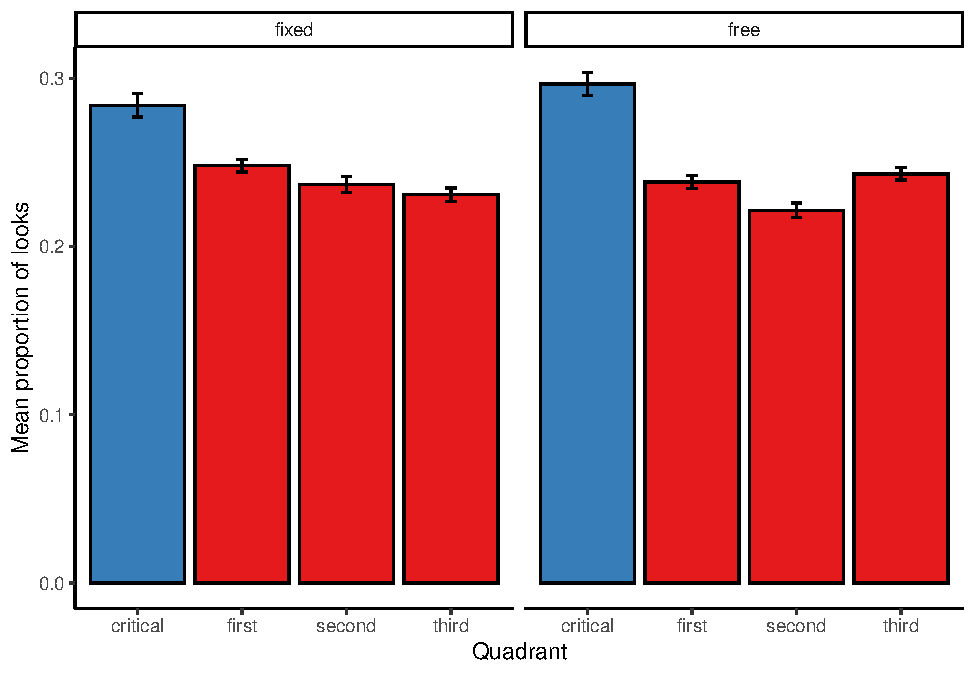
\includegraphics{manuscript_files/figure-latex/E2-gaze-fig-both-conds-1.pdf}
\caption{\label{fig:E2-gaze-fig-both-conds}Proportion of eye-gaze to critical quadrant and other three quadrants during memory retrieval in a) fixed and b) free viewing conditions.}
\end{figure}

The proportion of looks across quadrants in the free-viewing condition was analyzed in linear mixed-effects model with quadrant as the predictor (critical as the reference level). The model included random intercepts and slopes for participants\footnote{ \texttt{lme4} syntax: \texttt{lmer(proportion\ \textasciitilde{}\ quadrant\ +\ (1+quadrant\textbar{}subject\_id))}. Among other limitations, this approach violates the independence assumptions of the linear model because looks to the four locations are not independent. This analysis was chosen because it is analogous to the ANOVA analysis conducted in the original paper.} Proportions of looks were significantly higher for the critical quadrant compared to the other three (first: \emph{b} = -0.06, \emph{SE} = 0.01, \emph{p}\textless0.001, second: \emph{b} = -0.08, \emph{SE} = 0.01, \emph{p}\textless0.001, third: \emph{b} = -0.05, \emph{SE} = 0.01, \emph{p}\textless0.001 )

\begin{figure}
\centering
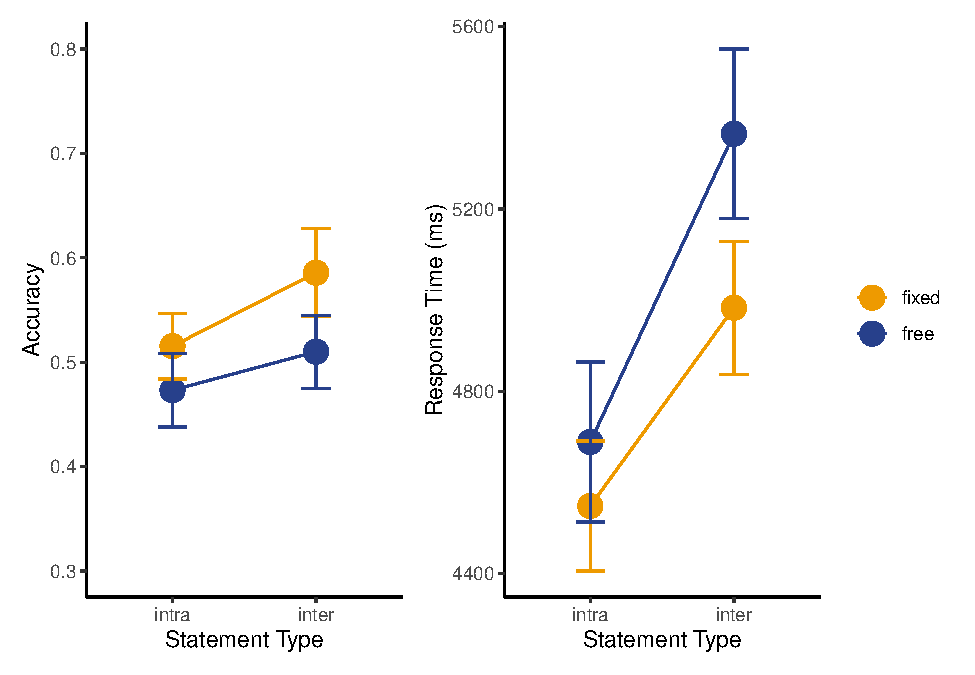
\includegraphics{manuscript_files/figure-latex/E2-rt-acc-fig-1.pdf}
\caption{\label{fig:E2-rt-acc-fig}Accuracy and response times during memory retrieval.}
\end{figure}

\textbf{Response Time and Accuracy}. Participants' response times and accuracies on memory questions are summarized in Figure \ref{fig:E2-rt-acc-fig}.
Both dependent variables were analyzed with linear mixed-effects model with relation type (interobject = -0.5, intraobject=0.5) and viewing\_condition (fixed = -0.5, free=0.5) and their interaction as the predictors.
The model included random intercepts for participants\footnote{ \texttt{lme4} syntax: \texttt{lmer(DV\ \textasciitilde{}\ relation\_type*viewing\_condition\ +\ (1\textbar{}subject\_id))}}.
Accuracy did not differ significantly between interobject and intraobject questions (\emph{b} = -0.05, \emph{SE} = 0.03, \emph{p}=0.05). Participants were less accurate in the free viewing condition than the fixed condition (\emph{b} = -0.06, \emph{SE} = 0.03, \emph{p}=0.03).
Response times were slower for interobject (e.g., ``The train is to the right of the taxi.'') than intraobject (e.g., ``The train is facing right.'') questions (\emph{b} = -555.60, \emph{SE} = 105.24, \emph{p}\textless0.001). Response times were slower in the free viewing condition than the fixed condition (\emph{b} = 260.98, \emph{SE} = 105.24, \emph{p}\textless0.001).
The interaction was not a significant predictor for response times or accuracy.
These behavioral results are inconsistent with the original findings.

One possibility is that in-lab participants were much more compliant with the instruction to keep their gaze on central fixation (though these data are not reported in the original paper). When analyzing results from the subset of participants (N = 25) who were most compliant during the fixed-viewing block (at least 25\% of their looks fell within 20\% of the center of the display), the viewing condition effects and the interactions were not signficant. Given the smaller sample size we do not interpret these results further.

\emph{Q: Can we recover item IDs to do crossed random effects?}

\hypertarget{calibration-1}{%
\subsubsection{Calibration}\label{calibration-1}}

Participants' calibration quality, measured as the mean percentage of fixations that landed within 200 pixels of the calibration point, varied substantially (between 17.78 and 100 \%).
The quality of a participant's calibration was not significantly correlated with the participant's effect size ( \emph{Pearson's r}= 0.20, \emph{p} = 0.14) as measured by the difference between the proportion of looks to the critical quadrant minues the average proportion of looks to the average of the other three quadrants.

\hypertarget{discussion-1}{%
\subsection{Discussion}\label{discussion-1}}

\hypertarget{experiment-3}{%
\section{Experiment 3}\label{experiment-3}}

The third study was a replication attempt of
Manns, Stark, and Squire (2000) which aimed to show that the visual
paired-comparison task, widely used in the patient literature, tapped
into declarative memory. In the visual paired-comparison task, two
identical pictures were presented side by side for a brief viewing
period. After a delay, one of the previously viewed pictures was
presented along with a new picture. Individuals looked more at the new
picture than the old picture and the time spent looking was correlated
with later recognition memory performance. On the other hand perceptual
priming, thought to recruit non-declarative memory, was not linked to
later recognition. (The perceptual priming arm of the design was not
included in this replication.)

\hypertarget{methods-2}{%
\subsection{Methods}\label{methods-2}}

\hypertarget{participants-3}{%
\subsubsection{Participants}\label{participants-3}}

Our initial sample size was 51 participants for the first day of our
experiment and 48 of them came back for the second day. Following Manns
et al., we excluded 3 participants due to perfect performance on the
recognition memory test. Our final sample size was 45 participants.

\hypertarget{procedure-2}{%
\subsubsection{Procedure}\label{procedure-2}}

The task began with a 7-point eye-tracker calibration (each point was
presented 3 times in a random order) and validation with 3 points (each
presented once). The point locations were designed to focus calibration
on the center of the screen and the middle of the left and right halves
of the screen. The experiment was administered over the course of two
consecutive days. It consisted of three sections: a presentation phase,
a test phase, and a recognition test. The first two phases occurred on
the first day, while the recognition test occurred on the second day.

During the presentation phase, participants viewed 24 pairs of identical
color photographs depicting common objects. Each pair was presented for
5 seconds and an interval of 5 seconds elapsed before the next pair was
shown. The order of the photographs was randomized and different for
each participant. After completion of the presentation phase,
participants were given a 5-minute break during which they could look
away from the screen.

After the break, they were prompted to complete the eye-tracking
calibration again before beginning the test phase. During this phase,
participants again viewed 24 pairs of photographs with an interstimulus
duration of 5 seconds. In each pair, one photograph was previously seen
during the presentation phase, while the other was new. Which pictures
were old or new was counterbalanced across participants.
For half of the participants in each counterbalancing group, the new and
old photographs were
reversed.

Approximately 24 hours after completing the first session, with a leeway
interval of 12 hours to accommodate busy schedules, participants were
given the recognition test. It consisted of 48 photographs, presented
one at a time. Each was shown on the screen for 1 second, followed by a
1 second interstimulus interval. Half of the pohotographs had been
viewed twice on the previous day and were deemed the ``targets.'' The
other half depicted an object with the same name as an object in one of
the old photographs, but had not been viewed before, deemed ``foils.''
Each photograph remained on the screen until the participants indicated
whether or not they had seen it before by pressing `y' for yes and `n'
for no. After they pressed one of the two keys, a prompt on the screen
asked them to rate their confidence in their answer from 1 as a ``pure
guess'' to 5 as ``very sure.'' by clicking on the corresponding number on
the screen. No feedback on their responses was given during the test.

The experimental design is visually depicted in Figure XX

\hypertarget{materials}{%
\subsubsection{Materials}\label{materials}}

Images were selected XXX\ldots{}

There were two modifications we made to the methods of the original
experiment. As we are only replicating the declarative memory component
of the original experiment, we did not have a ``priming group.''
Therefore, we followed only the procedure for the ``looking group.''
Additionally, for each section of the study, the stimuli was presented
on a single screen instead of two screens due to the constraints of the
online experiment format.

\hypertarget{data-analysis-1}{%
\subsubsection{Data analysis}\label{data-analysis-1}}

\hypertarget{results-2}{%
\subsection{Results}\label{results-2}}

\hypertarget{day-1}{%
\paragraph{Day 1}\label{day-1}}

During day 1 of the experiment, participants viewed pairs of images, one of which was always familiar and the other unfamiliar. We calculated a looking score for each participant, defined as the proportion of gaze samples in the ROI of the unfamiliar image out of all the gaze samples that were in either ROI. Gaze samples that were not in either ROI were not included in this analysis. A looking score of 0.5 indicates that participants looked equally often at the familiar and unfamiliar images, while a looking score above 0.5 indicates a preference for the unfamiliar object and a looking score below 0.5 indicate a preference for the familiar object.

Of the 1248 trials in the experiment, 78 had no fixations in either ROI, and so the looking score was unknown. We removed these trials from this analysis.

The mean looking score was 0.55 (\emph{SD} = 0.10). This significantly greater than 0.5, \emph{t}(49) = 3.29, \emph{p} = 0.00, indicating that participants did show a preference for looking at the novel objects.

\begin{figure}
\centering
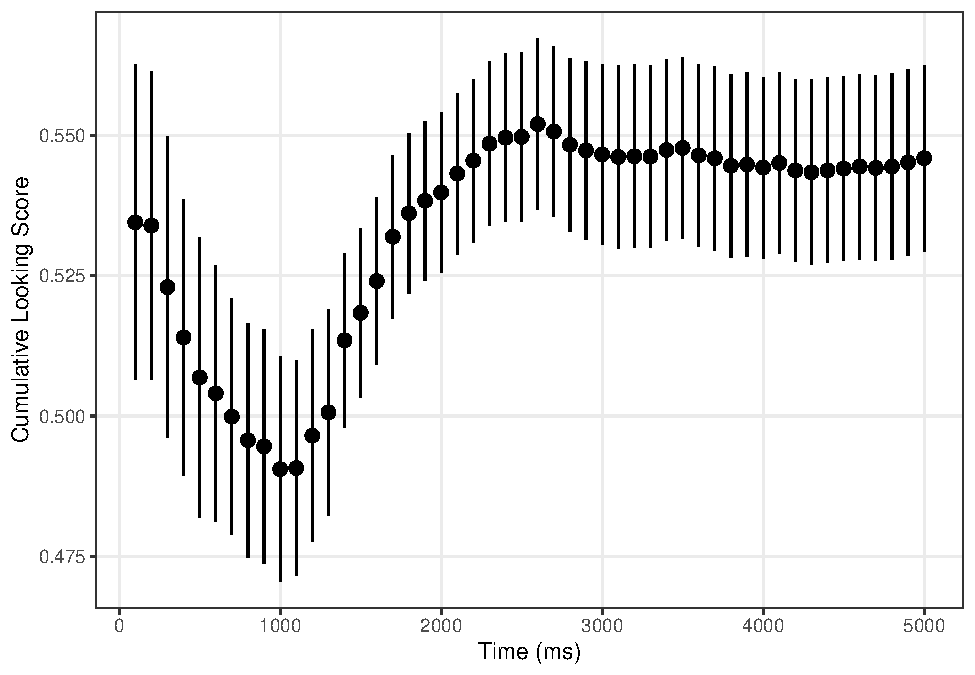
\includegraphics{manuscript_files/figure-latex/Plot of cumulative looking score-1.pdf}
\caption{(\#fig:Plot of cumulative looking score)Cumulative looking score over the 5 second exposure during part 2 of day 1. Error bars represent +/- 1 SEM.}
\end{figure}

\hypertarget{day-2}{%
\paragraph{Day 2}\label{day-2}}

In all of these analyses, we excluded the 16 (out of 2304) trials where the response time for the recognition judgment was greater than 10 seconds.

Participants correctly identified whether the image was familiar or unfamiliar 87.09\% (\emph{SD} = 10.49) of the time. After excluding the 3 participants who responded correctly to all images, the average confidence rating for correct responses (M = 3.51; SD = 0.41) was significantly higher than their average confidence ratings for incorrect responses (M = 2.55; SD = 0.75), t(44) = -9.36, p = 0.00 . Among the same subset of participants, response times for correct responses (M = 1,443.49, SD = 413.94) were also significantly faster than for incorrect responses (M = 2,212.65, SD = 1,733.76), t(44) = 3.43 , p = 0.00.

To see whether preferentially looking an the unfamiliar object on day 1 was correlated with confidence and response time for correct responses on day 2, we computed the correlation coefficient between day 1 looking scores and day 2 confidence/RT for each participant. Following the original analysis, we transformed these values using the Fisher p-to-z transformation. Using one-sample t-tests, we found no significant different from 0 for the correlation between looking score and confidence ratings, t(38) = 0.46, p = 0.65 (excluding the subjects who gave the same confidence judgment for all images), nor the the correlation between looking score and RT, t(46) = 0.49, p = 0.63.

\begin{verbatim}
## Warning: Removed 75 rows containing missing values (geom_point).
\end{verbatim}

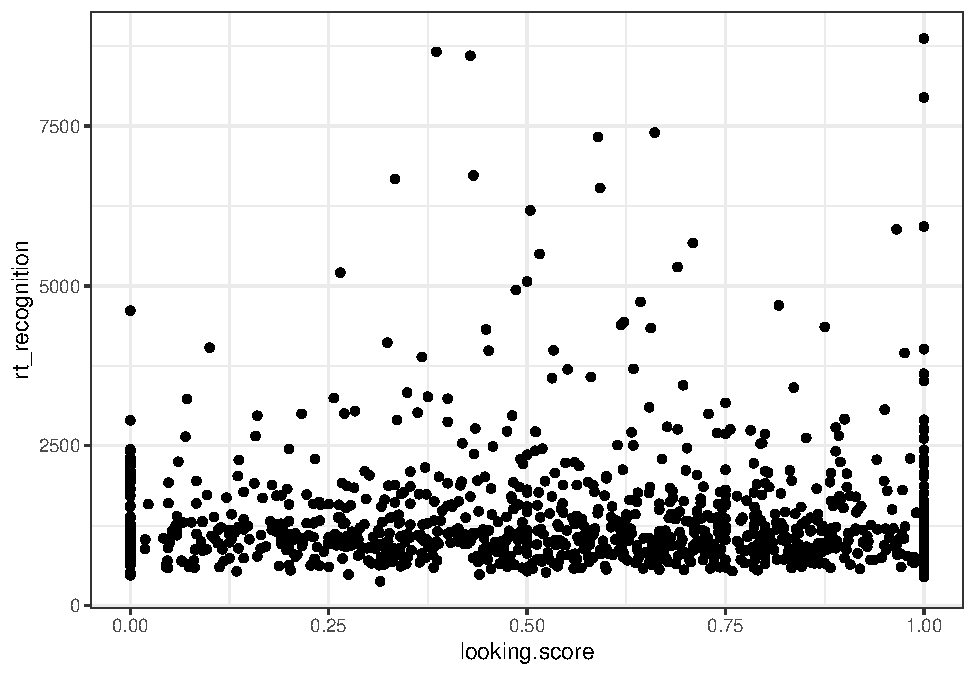
\includegraphics{manuscript_files/figure-latex/Plot Looking Score Correlations-1.pdf}

\hypertarget{effects-of-rois}{%
\subsubsection{Effects of ROIs}\label{effects-of-rois}}

In the original experiment, the two objects on day 1 were presented on two separate monitors and gaze was coded by manually coding video recordings. In our replication analysis, we analyzed eye movement data using ROIs defined around the two images. In this section we explore an alternative coding of the eye movement data by coding simply left half vs.~right half of the screen. The coarser coding may be more appropriate for webcam-based eyetracking.

The correlation between looking scores using the ROI method and the halves method is 0.76.

\begin{figure}
\centering
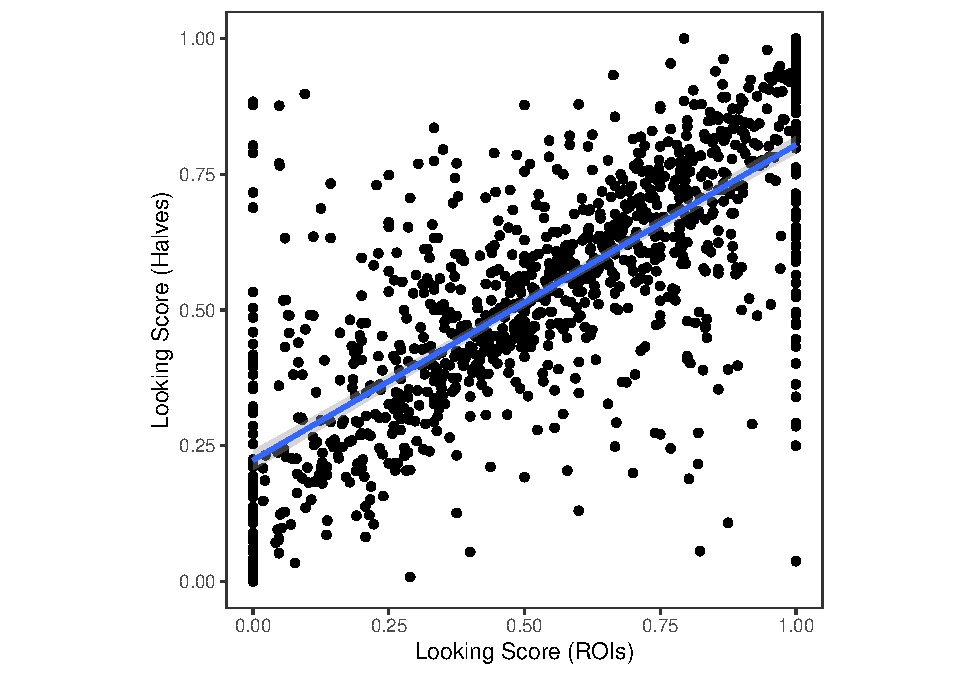
\includegraphics{manuscript_files/figure-latex/E3-roi correlation of looking score-1.pdf}
\caption{(\#fig:E3-roi correlation of looking score)Correlation between looking scores calculated using ROIs and using screen halves.}
\end{figure}

\hypertarget{looking-scores}{%
\paragraph{Looking Scores}\label{looking-scores}}

When looking scores are coded as left vs.~right half of the screen, we find that participants looked more at the novel object. The mean looking score was 0.54 (\emph{SD} = 0.08). This was significantly greater than 0.5, \emph{t}(50) = 3.51, \emph{p} = 0.00.

\begin{figure}
\centering
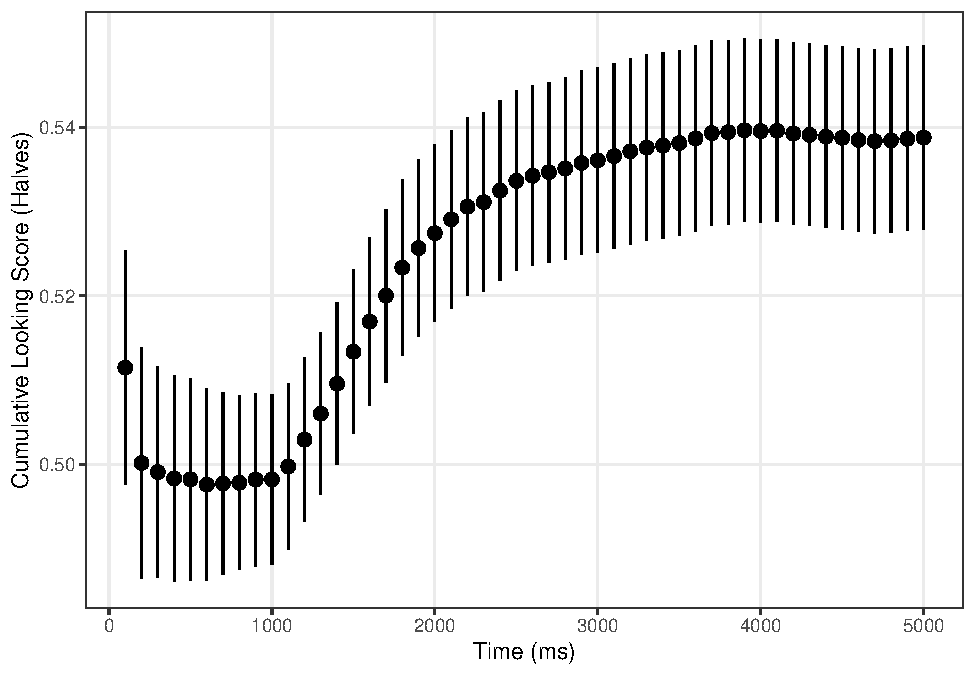
\includegraphics{manuscript_files/figure-latex/E3-roi Plot of cumulative looking score-1.pdf}
\caption{(\#fig:E3-roi Plot of cumulative looking score)Cumulative looking score over the 5 second exposure during part 2 of day 1. Error bars represent +/- 1 SEM.}
\end{figure}

\hypertarget{correlations-with-day-2-performance}{%
\paragraph{Correlations with Day 2 Performance}\label{correlations-with-day-2-performance}}

Performance on day 2 remained uncorrelated with day 1 looking scores after switching the coding of gaze. We found no significant different from 0 for the correlation between looking score and confidence ratings, t(39) = 0.74, p = 0.47 (excluding the subjects who gave the same confidence judgment for all images), nor the the correlation between looking score and RT, t(47) = 0.28, p = 0.78.

\hypertarget{calibration-2}{%
\subsubsection{Calibration}\label{calibration-2}}

\hypertarget{calibration-accuracy}{%
\paragraph{Calibration Accuracy}\label{calibration-accuracy}}

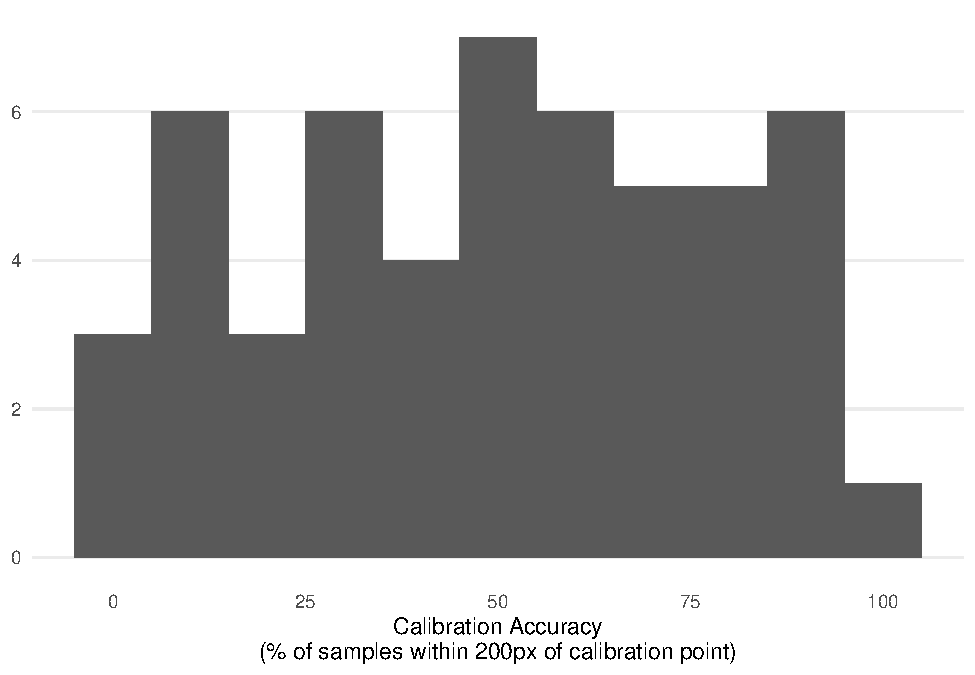
\includegraphics{manuscript_files/figure-latex/E3-cal Plot Calibration Accuracy-1.pdf}

\hypertarget{correlation-with-effects}{%
\paragraph{Correlation with Effects}\label{correlation-with-effects}}

To see if calibration success is correlated with the eye tracking effects, we calculated a calibration score for each participant. The calibration score was the average proportion of samples within XXX pixels of the validation points during the final validation phase before the eye tracking is performed.

Calibration scores were not correlated with looking scores, regardless of which method was used to calculate looking scores.

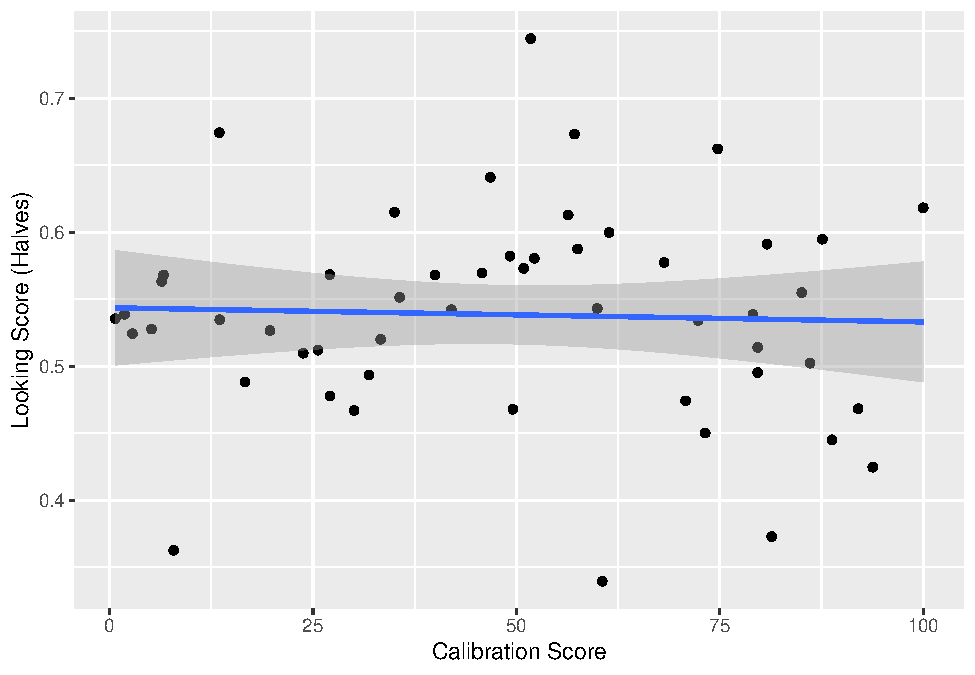
\includegraphics{manuscript_files/figure-latex/E3-cal Plot looking score (halves) by calibration-1.pdf}

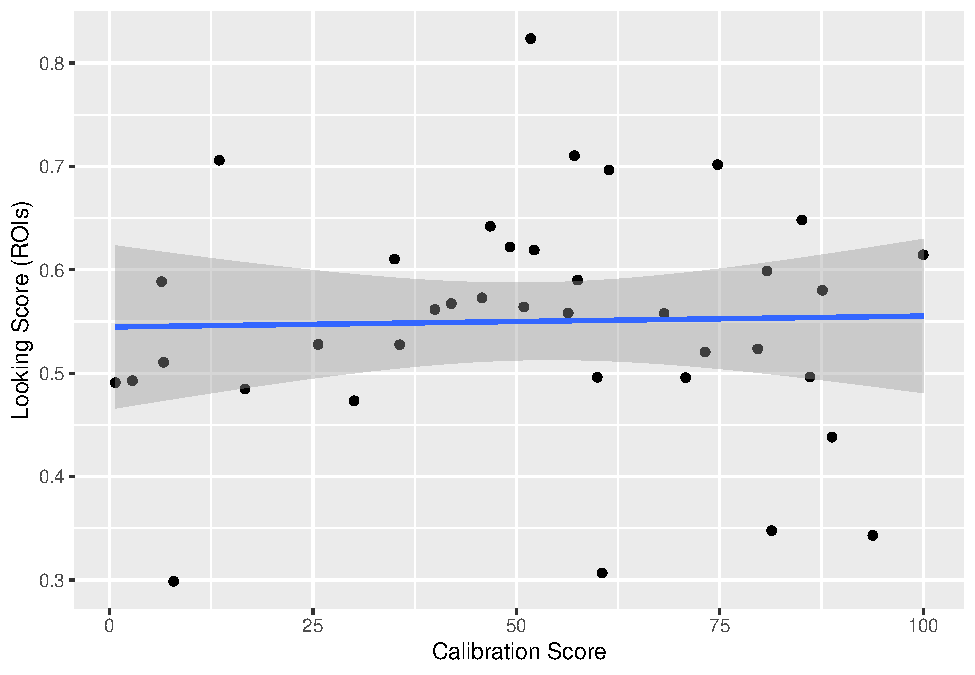
\includegraphics{manuscript_files/figure-latex/E3-cal Plot looking score (roi) by calibration-1.pdf}

We then looked at the correlation of calibration scores with the correlation between day 2 memory performance and day 1 looking scores for both kinds of behavioral and looking measures. None of the four relationships showed a significant correlation.

\includegraphics{manuscript_files/figure-latex/E3-cal Plot correlations with calibration score-1.pdf}

\hypertarget{discussion-2}{%
\subsection{Discussion}\label{discussion-2}}

\hypertarget{experiment-4}{%
\section{Experiment 4}\label{experiment-4}}

The fourth study was a replication attempt of Experiment 1 in
Ryskin, Qi, Duff, and Brown-Schmidt (2017), which was closely modeled on
Snedeker and Trueswell (2004). These studies used the
visual world paradigm to show that listeners use knowledge of the
co-occurrence statistics of verbs and syntactic structures to resolve
ambiguity. For example, in a sentence like ``Feel the frog with the
feather,'' the phrase ``with the feather'' could be describing the frog, or
it could be describing the instrument that should be used to do the
``feeling.'' When both options (a frog holding a feather and a feather by
itself) are available in the visual display, listeners rely on the
verb's ``bias'' (statistical co-occurrence either in norming or corpora)
to rapidly choose an action while the sentence is unfolding. .

\hypertarget{methods-3}{%
\subsection{Methods}\label{methods-3}}

The stimuli, experimental code, and data and analysis scripts can be
found on the Open Science Framework at the following link,
\url{https://osf.io/x3c49/} (\url{https://osf.io/x3c49/}). The pre-registration
for the study can be found at \url{https://osf.io/3v4pg}
(\url{https://osf.io/3v4pg}).

\hypertarget{participants-4}{%
\subsubsection{Participants}\label{participants-4}}

58 (??) participants were paid \$XX for their participation
. A sample size of 58 was chosen because we wanted to
replicate the experiment with greater statistical power. Note that the
original study had a sample size of 24.

\hypertarget{procedure-3}{%
\subsubsection{Procedure}\label{procedure-3}}

\begin{itemize}
\tightlist
\item
  \emph{TO DO:} add details of calibration point locations
\end{itemize}

After the eye-tracking calibration, participants went through an audio
test so they could adjust the audio on their computer to a comfortable
level. Before beginning the experiment, they were given instructions
that four objects would appear, an audio prompt would play, and they
should do their best to use their mouse to act out the instructions.
They then went through three practice trials which were followed by 54
critical trials and 24 filler trials presented in a random order.

During a trial, four pictures were displayed (target animal, target
instrument, distractor animal, distractor instrument), one in each
corner of the screen, and participants heard an audio prompt that
contained instructions about the action they needed to act out (e.g.,
``Rub the butterfly with the crayon''; see Figure XX)\footnote{In the original study, the pictures appeared one by one on the
  screen and their names were played as they appeared. We removed this
  introductory portion of the trial to save time}. Using their
cursor, participants could act out the instructions by clicking on
objects and moving them or motioning over the objects\footnote{As opposed to the original study we recorded mouse movement
  instead of clicking behavior since not all of the audio prompts
  required clicking. For example, the sentence ``locate the camel with
  the straw'' may not involve any clicking but rather only mousing over
  the camel.}. After the
action was completed, the participants were instructed to press the
space bar which led to a screen that said ``Click Here'' in the middle in
order to remove bias in the eye and mouse movements from the previous
trial. The experiment only allowed the participants to move on to the
next trial once the audio was completely done playing and the mouse had
been moved over at least one object.

\textcolor{red}{TO DO: ADD FIGURES Figure 1: An example of a critical trial for the sentence “Rub the butterfly with the crayon.” The butterfly is the target animal, the panda is the distractor animal, the crayon is the target instrument, and the violin is the distractor instrument.}

\hypertarget{materials-1}{%
\subsubsection{Materials}\label{materials-1}}

The images and audios presented to the participants were the same
stimuli used in the original study (available here ). The critical
trials were divided into modifier-biased, instrument-biased, and
equibiased conditions, and the filler trials did not contain ambiguous
instructions. Two lists of critical trials were made with different verb
and instrument combinations (e.g., ``rub'' could be paired with ``panda''
and ``crayon'' in one list and ``panda'' and ``violin'' in the second list).
Within each list, the same verb was presented twice but each time with a
different target instrument and animal. The lists were randomly assigned
to the participants to make sure the effects were not caused by the
properties of the animal or instrument images used. The list of verbs
used can be found in Appendix A of the original study.

\hypertarget{results-3}{%
\subsection{Results}\label{results-3}}

\hypertarget{replication-2}{%
\subsubsection{Replication}\label{replication-2}}

The location of initial mouse movements was used to assess whether the final interpretation of ambiguous sentences was biased by the verb. Figure \ref{fig:E4-mouse-moves-fig} suggests that listeners were more likely to move their mouse first over the target instrument when the verb was equi-biased than when the verb was modifier-biased and even more so when the verb was instrument-biased. The opposite graded pattern can be observed for mouse movements over the target animal.

\begin{figure}
\centering
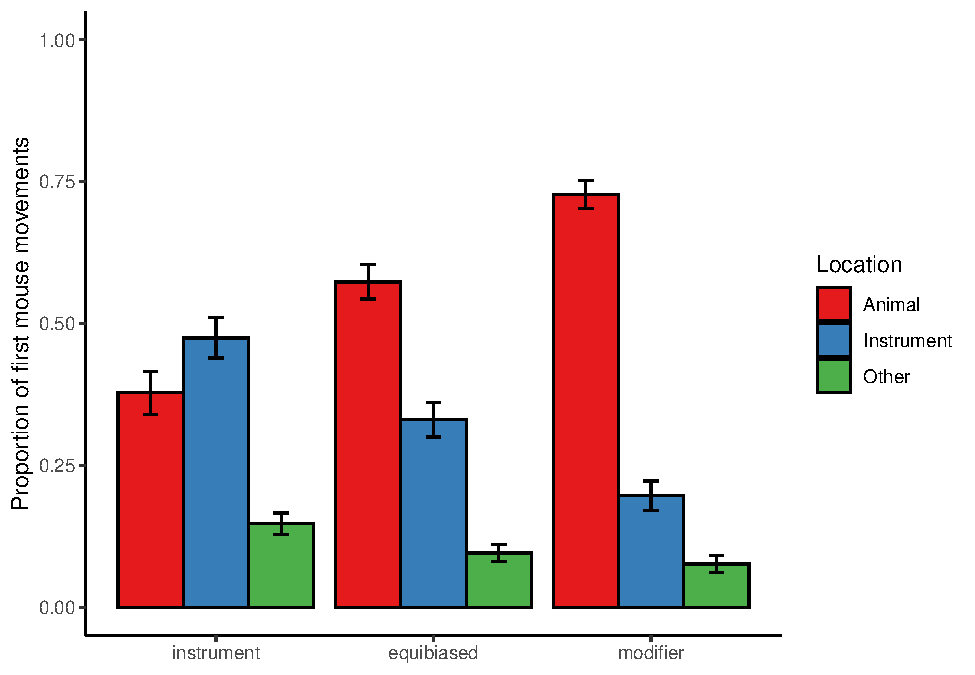
\includegraphics{manuscript_files/figure-latex/E4-mouse-moves-fig-1.pdf}
\caption{\label{fig:E4-mouse-moves-fig}Proportion of first mouse movements by location and verb bias.}
\end{figure}

A mixed-effects logistic regression model was used to predict whether the first movement was on the target instrument with the verb bias condition as an orthogonally contrast-coded (instrument vs.~equi \& modifier: inst = -2/3, equi = 1/3, mod = 1/3; equi vs.~modifier: inst = 0, equi = -1/2, mod = 1/2 ) fixed effect. Participants and items were entered as varying intercepts with by-participant varying slopes for verb bias condition\footnote{\texttt{lme4} syntax: \texttt{glmer(is.mouse.over.instrument\ \textasciitilde{}\ verb\_bias\ +\ (1\ +\ verb\_bias\ \textbar{}\ participant)\ +\ (1\ \textbar{}\ item),\ family="binomial",\ data=d)}}. Participants were more likely to first move their mouse over target instruments in the instrument-biased condition relative to the equi-biased and modifier-biased condition (\emph{b} = -1.50, \emph{SE} = 0.25, \emph{p} \textless{} 0.01). Further, participants were more likely to first move their mouse over target instruments in the equi-biased condition relative to the modifier-biased condition (\emph{b} = -1.10, \emph{SE} = 0.29, \emph{p} \textless{} 0.01)

Gaze fixations were time-locked to the auditory stimulus on a trial by trial basis and categorized as being directed towards one of the four items in the display if the x, y coordinates fell within a rectangle containing the image. Figure \ref{fig:E4-gaze-timecourse-fig} suggests that the participants made more fixations to the target animal when the verb was modifier-biased compared to when the the verb was equi-biased and they looked at the target animal least when the verb was instrument-biased. The pattern was reversed for looks to the target instrument.

\begin{figure}
\centering
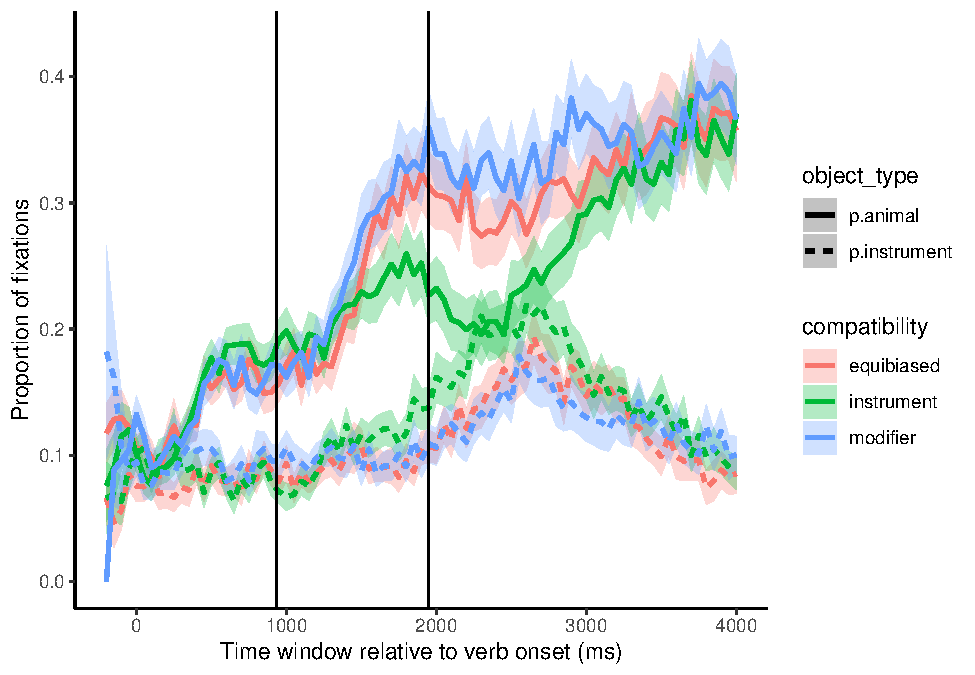
\includegraphics{manuscript_files/figure-latex/E4-gaze-timecourse-fig-1.pdf}
\caption{\label{fig:E4-gaze-timecourse-fig}Timecourse of eye-gaze to target animal and target instrument by verb bias condition. Vertical lines indicate average onsets of animal and instrument offset by 200ms.}
\end{figure}

In order to assess how verb bias impacted sentence disambiguation as the sentence unfolded, the proportion of fixations was computed in three time windows: the verb-to-animal window (from verb onset + 200 ms to animal onset + 200 ms), the animal-to-instrument window (from animal onset + 200 ms to instrument onset + 200 ms), and the post-instrument window (from instrument onset + 200 ms to instrument onset + 1500ms + 200 ms). Mixed-effects linear regression models were used to predict the proportions of fixations to the target animal within each time window with the verb bias condition as an orthogonally contrast-coded (instrument vs.~equi \& modifier: inst = -2/3, equi = 1/3, mod = 1/3; equi vs.~modifier: inst = 0, equi = -1/2, mod = 1/2 ) fixed effect. Participants and items were entered as varying intercepts\footnote{\texttt{lme4} syntax: \texttt{lmer(prop.fix.target.animal\ \textasciitilde{}\ verb\_bias\ +\ (1\ +\ verb\_bias\ \textbar{}\ participant)\ +\ (1\ \textbar{}\ item),\ data=d)}. A model with by-participant varying slopes for verb bias condition was first attempted but did not converge.}. In the \emph{verb-to-noun} window, participants did not look more at the target animal in any of the verb bias conditions (Instrument vs.~Equi and Modifier: \emph{b} = -0.01, \emph{SE} = 0.02, \emph{p} = 0.59; Equi vs.~Modifier: \emph{b} = 0, \emph{SE} = 0.02, \emph{p} = 1 ). In the \emph{noun-to-instrument} window, participants looked more at the target animal in the modifier-biased condition and equi-biased conditions relative to the instrument-biased condition ( \emph{b} = 0.03, \emph{SE} = 0.01, \emph{p} \textless{} 0.01) and in the modifier biased relative to the equi-biased condition ( \emph{b} = 0.02, \emph{SE} = 0.01, \emph{p} \textless{} 0.05). In the \emph{post-instrument} window, participants looked more at the target animal in the modifier-biased condition and the equi-biased conditions relative to the instrument-biased condition ( \emph{b} = 0.08, \emph{SE} = 0.02, \emph{p} \textless{} 0.01) but not significantly so in the modifier biased condition relative to the equi-biased condition ( \emph{b} = 0.03, \emph{SE} = 0.02, \emph{p} = 0.15).

\hypertarget{comparison-to-in-lab-data-1}{%
\subsubsection{Comparison to in-lab data}\label{comparison-to-in-lab-data-1}}

The web version of the study qualitatively replicates the action and eye-tracking results of the original dataset (Ryskin et al., 2017).
The mouse click results from both studies are summarized in Figure \ref{fig:E4-mouse-moves-fig-web-and-orig}.
The quantitative patterns of clicks were similar to those observed in the original dataset, though for Instrument-biased verbs, clicks were closer to evenly split between the animal and the instrument relative to the in-lab study where they were very clearly biased toward the instrument.

\begin{figure}
\centering
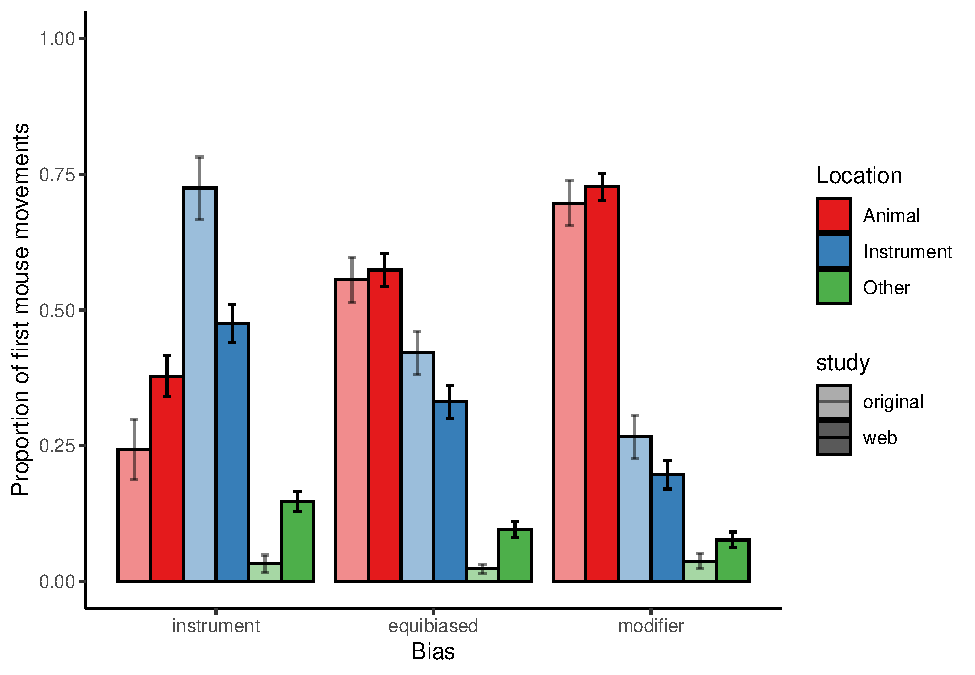
\includegraphics{manuscript_files/figure-latex/E4-mouse-moves-fig-web-and-orig-1.pdf}
\caption{\label{fig:E4-mouse-moves-fig-web-and-orig}Proportion of first mouse movements by location and verb bias in the original dataset (Ryskin et al., 2017) and the current data collected online.}
\end{figure}

The eye-tracking results from both studies are summarized in Figure \ref{fig:E4-proportion-fix-by-window-both}.
For simplicity, and to reflect the dependent variable used in analyses, we average the proportion of fixations to the target animal within each time window.
Though the qualitative patterns are replicated, proportions of fixations to the target animal were much lower in the web version of the study.
This may reflect the fact that participants in the web study are less attentive and/or the quality of the webgazer eye-tracking system is lower, relative to the Eyelink 1000 which was used for the original study.

\begin{figure}
\centering
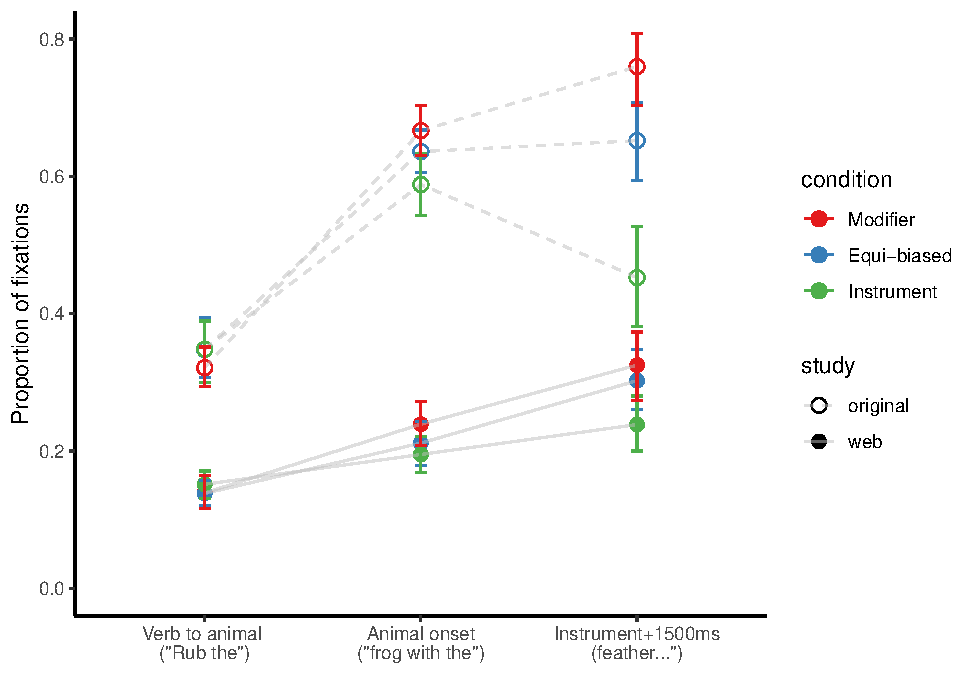
\includegraphics{manuscript_files/figure-latex/E4-proportion-fix-by-window-both-1.pdf}
\caption{\label{fig:E4-proportion-fix-by-window-both}Proportion of target fixations by verb bias in the original dataset (Ryskin et al., 2017) and the current data collected online. Error bars reflect bootstrapped 95\% CIs over subject means}
\end{figure}

\hypertarget{calibration-3}{%
\subsubsection{Calibration}\label{calibration-3}}

Participants' calibration quality, measured as the mean percentage of fixations that landed within 200 pixels of the calibration point, varied substantially (between 2.22 and 97.36 \%).
The quality of a participant's calibration significantly correlated with the participant's effect size ( \emph{Pearson's r}= 0.29, \emph{p} \textless{} 0.05).
The difference in target animal fixation proportions between modifier and instrument conditions was higher for participants with better calibration

Replicating the linear mixed-effects analysis (in the post-instrument onset time window only) on a subset of 35 participants with calibration quality \textgreater50\% suggests that the effect of verb bias condition was larger in this subset than in the full dataset. Participants looked more at the target animal in the modifier-biased condition and the equi-biased conditions relative to the instrument-biased condition ( \emph{b} = 0.10, \emph{SE} = 0.02, \emph{p} \textless{} 0.001) but not significantly so in the modifier biased condition relative to the equi-biased condition ( \emph{b} = 0.02, \emph{SE} = 0.02, \emph{p} = 0.29).

Replicating the linear mixed-effects analysis (in the post-instrument onset time window only) on a subset of 19 participants with calibration quality \textgreater75\% suggests that the effect of verb bias condition was larger in this subset than in the full dataset.
Participants looked more at the target animal in the modifier-biased condition and the equi-biased conditions relative to the instrument-biased condition ( \emph{b} = 0.11, \emph{SE} = 0.03, \emph{p} \textless{} 0.001) but not significantly so in the modifier biased condition relative to the equi-biased condition ( \emph{b} = 0.05, \emph{SE} = 0.03, \emph{p} = 0.13).

\hypertarget{effects-of-rois-1}{%
\subsubsection{Effects of ROIs}\label{effects-of-rois-1}}

Eye-tracking on the web differs critically from in-lab eye-tracking in that the size of the display differs across participants. Thus the size of the ROIs differs across participants. The current version of the web experiment used a bounding box around each image to determine the ROI.
This approach is flexible and accomodates variability in image size, but may exclude looks that are directed at the image but fall outside of the image (due to participant or eye-tracker noise) as show in Figure \ref{fig:E4-example-subj-looks-ROI}a. Alternatively, The display can be split into 4 quadrants which jointly cover the entire screen (see Figure \ref{fig:E4-example-subj-looks-ROI}b).

\begin{figure}
\centering
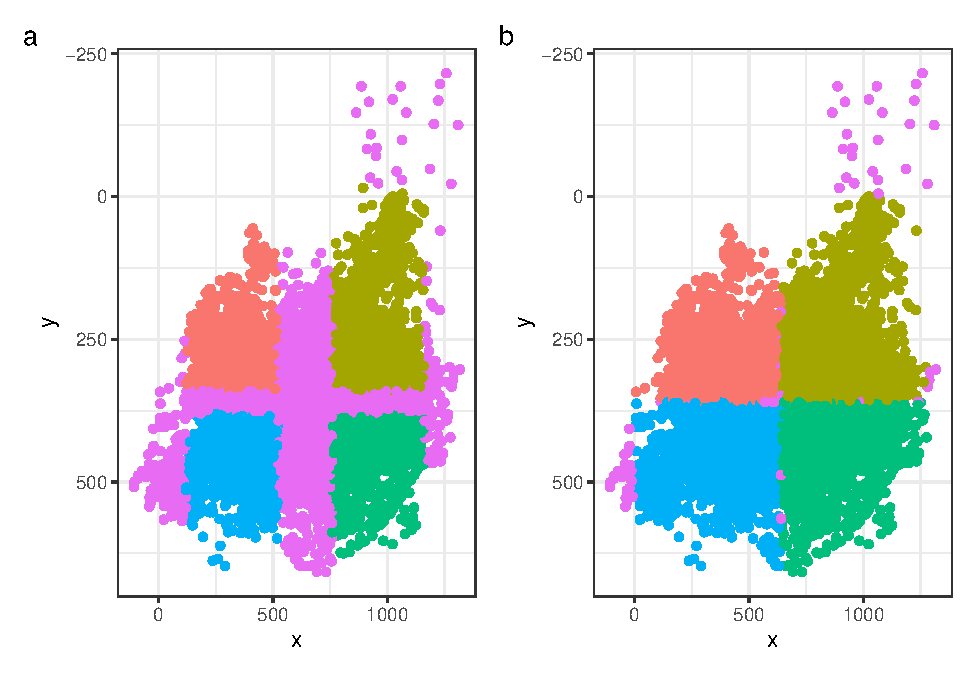
\includegraphics{manuscript_files/figure-latex/E4-example-subj-looks-ROI-1.pdf}
\caption{\label{fig:E4-example-subj-looks-ROI}Example participant's gaze coordinates categorized into ROIs based on a) image bounding boxes and b) screen quadrants. Magenta points indicate looks that were not categorized into an ROI}
\end{figure}

\begin{figure}
\centering
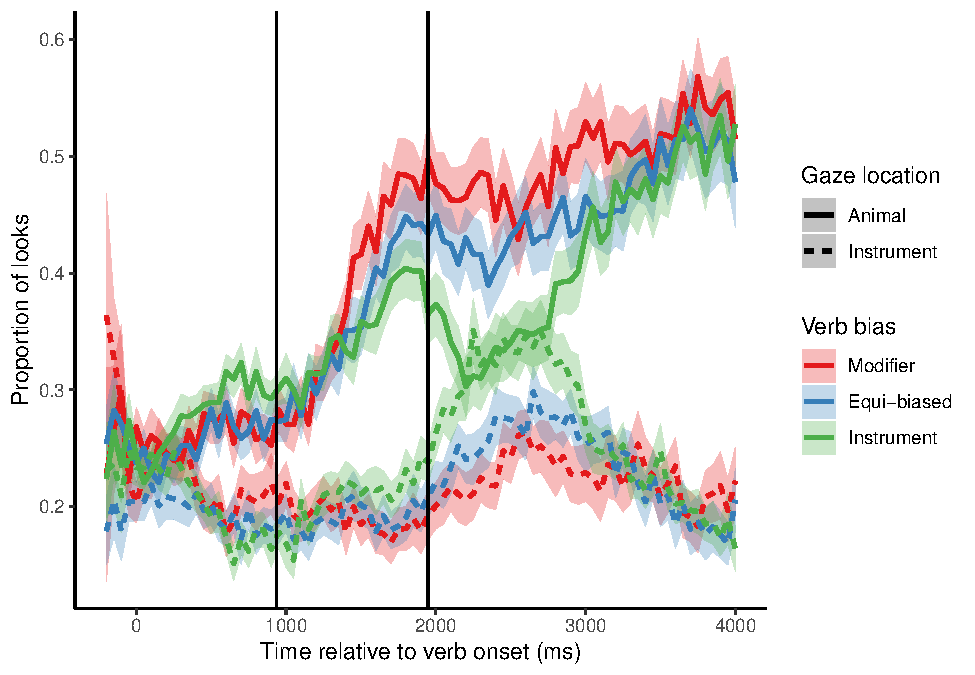
\includegraphics{manuscript_files/figure-latex/E4-gaze-timecourse-fig-quadrants-1.pdf}
\caption{\label{fig:E4-gaze-timecourse-fig-quadrants}Timecourse of eye-gaze to target animal and target instrument by verb bias condition with gaze categorized based on which quadrant of the screen the coordinates fall in (as opposed to a bounding box around the image). Vertical lines indicate average onsets of animal and instrument offset by 200ms.}
\end{figure}

Categorizing gaze location based on which of the four quadrants of the screen the coordinates fell in, increases the overall proportions of fixations (see Figure \ref{fig:E4-gaze-timecourse-fig-quadrants}). In the \emph{post-instrument} window, participants looked more at the target animal in the modifier-biased condition and the equi-biased conditions relative to the instrument-biased condition ( \emph{b} = 0.08, \emph{SE} = 0.02, \emph{p} \textless{} 0.01) and marginally so in the modifier biased condition relative to the equi-biased condition ( \emph{b} = 0.04, \emph{SE} = 0.02, \emph{p} = 0.05). Effect size estimates appeared somewhat larger and noise was somewhat reduced when using the quadrant categorization relative to the bounding box-based ROIs.

\hypertarget{discussion-3}{%
\subsection{Discussion}\label{discussion-3}}

\hypertarget{experiment-5}{%
\section{Experiment 5}\label{experiment-5}}

The fifth study was a replication attempt of Shimojo, Simion, Shimojo, and Scheier (2003),
which found that human gaze is actively involved in preference
formation. Separate sets of participants were shown pairs of human faces
and asked either to choose which one they found more attractive or which
they felt was rounder. Prior to making their explicit selection,
participants were increasingly likely to be fixating the face they
ultimately chose, though this effect was significantly weaker for
roundness discrimination.

Note that Shimojo and colleagues compare five conditions, of which we
replicate only the two that figure most prominently in their
conclusions: the ``face-attractiveness-difficult task'' and the
``face-roundness task''.

\hypertarget{methods-4}{%
\subsection{Methods}\label{methods-4}}

All stimuli, experiment scripts, data, and analysis scripts are
available on the Open Science Framework at \url{https://osf.io/eubsc/}
(\url{https://osf.io/eubsc/}). The study pre-registration is available at
\url{https://osf.io/tv57s} (\url{https://osf.io/tv57s}).

\hypertarget{participants-5}{%
\subsubsection{Participants}\label{participants-5}}

50 participants for the main task were recruited on Prolific and were
paid \$XX. 8 subjects, 4 from the attractiveness task group and 4 from
the roundness task group, were excluded for incorrect validations.
After this
data exclusion, we ended up with 21 participants each for the
attractiveness task and the roundness task. The original sample size in
Shimojo et al.~(2003) was 10 participants total. \#\#\# Procedure and
Design

At the beginning of the experimental task, participants completed a
9-point eye-tracker calibration (each point appeared 3 times in random
order) and 3-point validation. The validation point appeared once at
center, middle left, and middle right locations in random order.

During each trial of the main task, two faces were displayed on the two
halves of the screen, one on the left and one on the right (as in Figure
XX). Participants were randomly assigned to one of two tasks:
attractiveness or shape judgment. In the attractiveness task,
participants were asked to chose the more attractice face in the pair
and in the shape judgment task participants were asked to pick the face
that appeared rounder. They pressed the ``a'' key on their keyboard to
select the face on the left and the ``d'' key to select the face on the
right. A fixation cross appeared in the center of the screen between
each set of faces. Participants were asked to look at this fixation
cross in order to reset their gaze in between trials (???). The order of
the 19 face pairs was random for each participant.

\hypertarget{materials-and-norming}{%
\subsubsection{Materials and Norming}\label{materials-and-norming}}

The faces in our replication were selected from a set of 1,000 faces
within the Flickr-Faces-HQ Dataset. (The face images used in Shimojo et
al.~were from the Ekman face database and the AR face database.) These
images were chosen because the person in each image was looking at the
camera with a fairly neutral facial expression and appeared to be over
the age of 18. 27 participants were recruited on Prolific to participate
in stimulus norming (for attractiveness). They were paid \$XX for
completing the experiment. Data from 3 participants was excluded because
their mode response made up more than 50\% of their total responses
, for a total of 24 participants
in the norming. They each viewed all 172 faces and were asked to rate
them on a scale from 1 (less attractive) to 7 (more attractive) using a
slider. Faces were presented one at a time and in a random order for
each participant. Following Shimojo et al., 19 face pairs were made by
matching two faces that had a difference in mean attractiveness ratings
that was 0.25 points or lower and that matched in gender, race, and age
group (young adult, adult, or older adult).

\hypertarget{data-analysis-2}{%
\subsubsection{Data analysis}\label{data-analysis-2}}

In the original study, a video-based eye tracker was used. The eye
movements of participants were recorded with a digital camera
downsampled to 33.3 Hz, with eye position was then determined
automatically with MediaAnalyzer software. In our study, subjects
supplied their own cameras, so hardware sampling rate varied. However,
data was collected at 20 Hz.{[}TODO - CONFIRM{]}

\hypertarget{results-4}{%
\subsection{Results}\label{results-4}}

Due to large variation in response time latency, Shimojo and colleagues analyzed eye gaze for the 1.67 seconds prior to the response. This duration was one standard deviation of the mean response time, ensuring that all timepoints analyzed have data from at least 67\% of trials. In our dataset, one standard deviation amounts to 1.85 seconds. We then binned eyegaze data into 50 ms bins rather than the 30 ms bins used by Shimojo and colleagues, reflecting the different sampling rates.



\begin{figure}
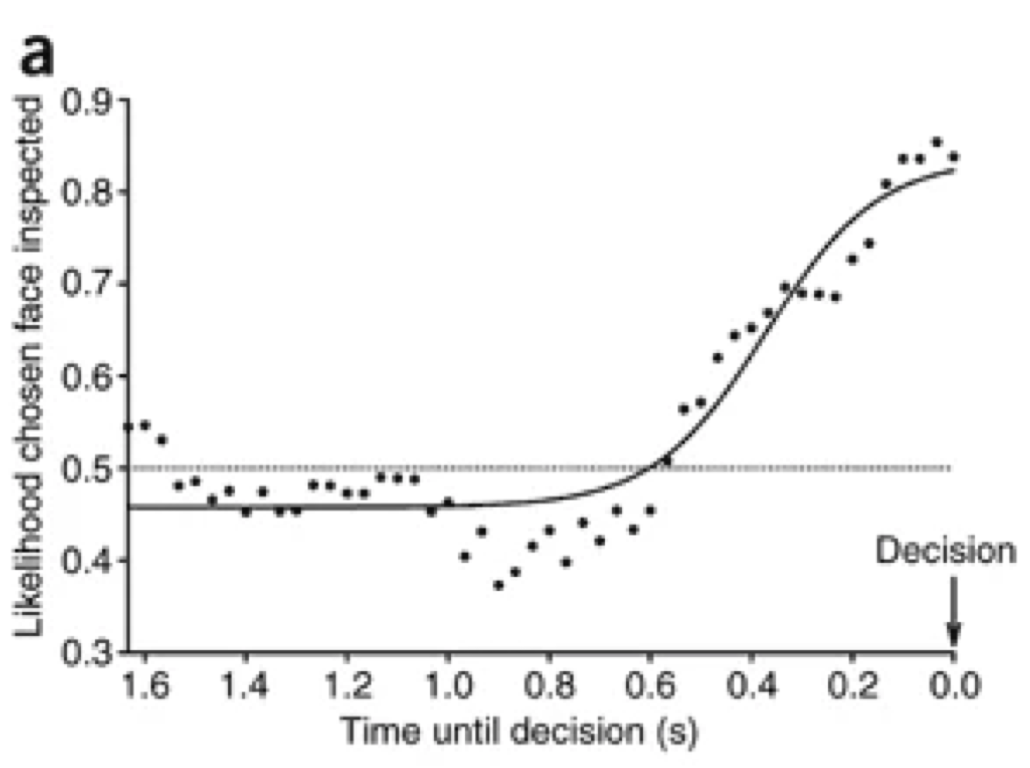
\includegraphics[width=0.45\linewidth]{figGroupEOrigA} 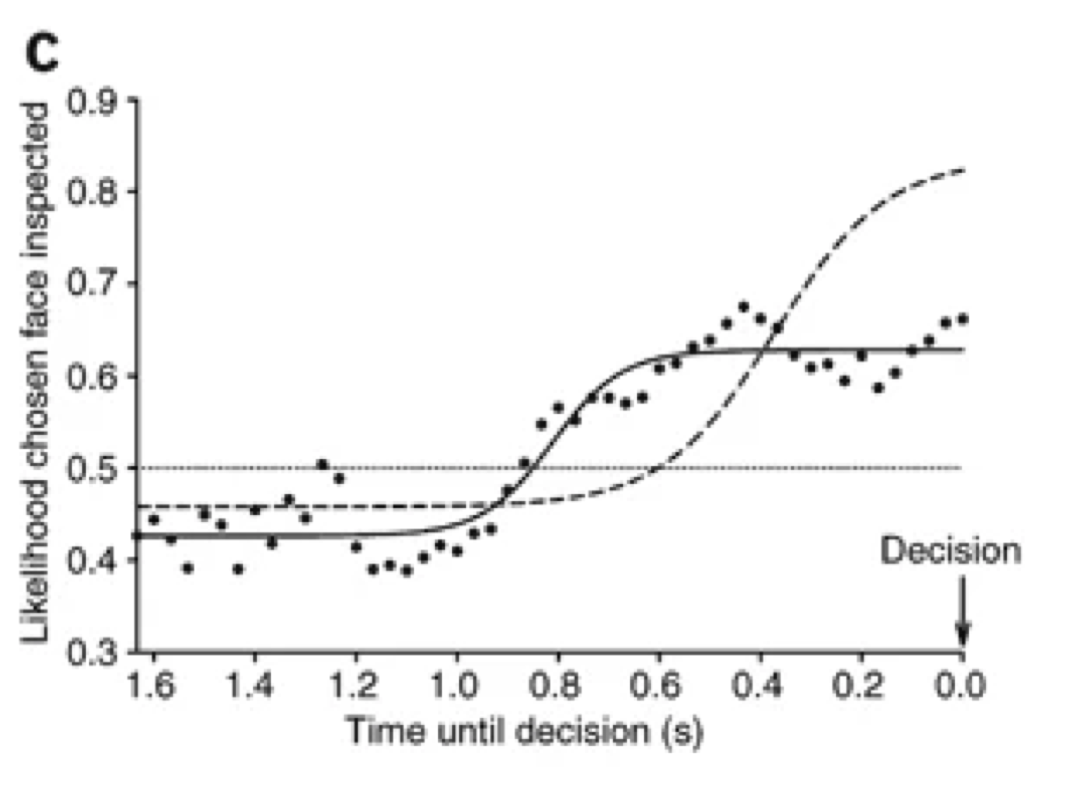
\includegraphics[width=0.45\linewidth]{figGroupEOrigB} \includegraphics[width=0.45\linewidth]{manuscript_files/figure-latex/groupEMain-3} \includegraphics[width=0.45\linewidth]{manuscript_files/figure-latex/groupEMain-4} \caption{Primary results from Exp. 5. \emph{Top} shows the original results from Shimojo and colleagues (Figures reprinted with permission{[}TODO{]}). The attractiveness judgment along with the best-fitting sigmoid is shown in the \emph{top left}. Results for the roundness judgment are show in the \emph{top right}, with the best-fitting sigmoid for the attractiveness judgment depicted in a dashed line for comparison (\emph{top right}). (\emph{Bottom}) shows the analogous results from the replication, with the attractiveness judgments on the \emph{bottom left} and the roundness judgments on the \emph{bottom right}. Again, the best-fitting sigmoid for the attractiveness judgments are plotted with a dashed line alongside the roundness results, for purposes of comparison.}\label{fig:groupEMain}
\end{figure}

Following Shimojo and colleagues, data for each condition were fit using a four-parameter sigmoid (Fig. \ref{fig:Shimojo}). These fit less well than in the original paper for both the attractiveness judgment (R\textsuperscript{2} = 0.84 vs.~0.91) and the roundness judgment (R\textsuperscript{2} = 0.54 vs.~0.91).

From these curves, Shimojo and colleagues focus on two qualitative findings. First, they note a higher asymptote for the attractiveness discrimination task relative to roundness discrimination. Qualitatively, this appears to replicate. However, their statistical analysis -- a Kolmogorov-Smirnov test for distance between two distributions -- is not significant (D = 0.19, p = 0.53), though it should be noted that this is a very indirect statistical test of the hypothesis and probably not very sensitive.

The second qualitative finding they note is that the curve for the roundness judgment ``saturates'' (asymptotes) earlier than the curve for the attractiveness judgment. They do not present any statistical analyses, but it is clear qualitatively that the result does not replicate.

\hypertarget{calibration-4}{%
\subsubsection{Calibration}\label{calibration-4}}

As in the previous experiments, calibration score was defined as the average proportion of samples within 200 pixels of the validation point during the final validation phase before the eye tracking is performed. The distribution across participants is shown in Fig. \ref{fig:E5cal}.


\begin{figure}
\includegraphics[width=0.45\linewidth]{manuscript_files/figure-latex/E5cal-1} \caption{Histogram of calibration success in Exp. 5. Where participants required more than one calibration (N=8), only the final calibration was considered.}\label{fig:E5cal}
\end{figure}

To determine whether calibration accuracy influenced our key effects, we calculated the percentage of samples during the task in which the participant was fixating the face they ultimately chose. There was a significant correlation for both the attractiveness judgments (r = 0.47 {[}0.04, 0.75{]}, p = 0.03) and the roundness judgments (r = 0.60 {[}0.23, 0.82{]}, p = 0). Inspection of Fig. \ref{fig:E5calcorr} reveals that this correlation is due to a handful of particpiants with calibration values below 50\%.



\begin{figure}
\includegraphics[width=0.8\linewidth]{manuscript_files/figure-latex/E5calcorr-1} \caption{Correlation between calibration accuracy (x-axis) and percentage of samples fixating target (y-axis) in Exp. 5.}\label{fig:E5calcorr}
\end{figure}

Thus, we re-analyzed the data, removing the participants whose calibration accuracy was not greater than 50\%. This slightly improved the fits of the sigmoids (Attractiveness: R\textsuperscript{2} = 0.79; Roundness: R\textsuperscript{2} = 0.60). However, the difference between sigmoids remained non-significant using the Kolmogorov-Smirnov test (D = 0.22, p = 0.35). Descriptively, the results do not look substantially different (Fig. \ref{fig:groupEMainrev}).



\begin{figure}
\includegraphics[width=0.45\linewidth]{manuscript_files/figure-latex/groupEMainrev-1} \includegraphics[width=0.45\linewidth]{manuscript_files/figure-latex/groupEMainrev-2} \caption{Revised results for Exp. 5 after removing low-calibration accuracy participants. \emph{Left}: Eyegaze during attractiveness judgments, along with the best-fitting sigmoid. \emph{Right}: Eyegze during roundness judgments, along with best-fitting sigmoid (best-fitting sigmoid for attractiveness is re-plotted with a dashed line for comparison).}\label{fig:groupEMainrev}
\end{figure}

\hypertarget{effects-of-rois-2}{%
\subsubsection{Effects of ROIs}\label{effects-of-rois-2}}

In the original experiment, eye gazes that did not directly fixate one or other of the faces were excluded. In this section we explore an alternative coding of the eye movement data by coding simply left half vs.~right half of the screen. The coarser coding may be more appropriate for webcam-based eyetracking.

Only a small percentage of samples (7.00\%) involved looks to anything other than one of the two faces. Thus, not surprisingly, the correlation between percentage of time spent fixating the to-be-chosen face using the ROI method and the halves method was near ceiling (r = 0.97 {[}0.97, 0.98{]}, p = 0). Since the choice of method had almost no effect on whether participants were coded as fixating one face or the other, we did not further investigate the effect of method choice on the analytic results.

\hypertarget{discussion-4}{%
\subsection{Discussion}\label{discussion-4}}

\hypertarget{combined-analyses}{%
\section{Combined Analyses}\label{combined-analyses}}

\begin{itemize}
\tightlist
\item
  Pooling data from all experiments we can look at patterns in the
  calibration and validation data
\end{itemize}

\hypertarget{general-discussion}{%
\section{General Discussion}\label{general-discussion}}

\newpage

\hypertarget{references}{%
\section{References}\label{references}}

\begingroup
\setlength{\parindent}{-0.5in}
\setlength{\leftskip}{0.5in}

\hypertarget{refs}{}
\begin{CSLReferences}{1}{0}
\leavevmode\vadjust pre{\hypertarget{ref-altmannIncrementalInterpretationVerbs1999}{}}%
Altmann, G. T. M., \& Kamide, Y. (1999). Incremental interpretation at verbs: Restricting the domain of subsequent reference. \emph{Cognition}, \emph{73}(3), 247--264. \url{https://doi.org/10.1016/S0010-0277(99)00059-1}

\leavevmode\vadjust pre{\hypertarget{ref-R-papaja}{}}%
Aust, F., \& Barth, M. (2020). \emph{{papaja}: {Create} {APA} manuscripts with {R Markdown}}. Retrieved from \url{https://github.com/crsh/papaja}

\leavevmode\vadjust pre{\hypertarget{ref-R-tinylabels}{}}%
Barth, M. (2022). \emph{{tinylabels}: Lightweight variable labels}. Retrieved from \url{https://cran.r-project.org/package=tinylabels}

\leavevmode\vadjust pre{\hypertarget{ref-R-lme4}{}}%
Bates, D., Mächler, M., Bolker, B., \& Walker, S. (2015). Fitting linear mixed-effects models using {lme4}. \emph{Journal of Statistical Software}, \emph{67}(1), 1--48. \url{https://doi.org/10.18637/jss.v067.i01}

\leavevmode\vadjust pre{\hypertarget{ref-R-Matrix}{}}%
Bates, D., \& Maechler, M. (2021). \emph{Matrix: Sparse and dense matrix classes and methods}. Retrieved from \url{https://CRAN.R-project.org/package=Matrix}

\leavevmode\vadjust pre{\hypertarget{ref-R-broom.mixed}{}}%
Bolker, B., \& Robinson, D. (2020). \emph{Broom.mixed: Tidying methods for mixed models}. Retrieved from \url{https://CRAN.R-project.org/package=broom.mixed}

\leavevmode\vadjust pre{\hypertarget{ref-R-shiny}{}}%
Chang, W., Cheng, J., Allaire, J., Sievert, C., Schloerke, B., Xie, Y., \ldots{} Borges, B. (2021). \emph{Shiny: Web application framework for r}. Retrieved from \url{https://CRAN.R-project.org/package=shiny}

\leavevmode\vadjust pre{\hypertarget{ref-deleeuwJsPsychJavaScriptLibrary2015}{}}%
de Leeuw, J. R. (2015). {jsPsych}: {A JavaScript} library for creating behavioral experiments in a {Web} browser. \emph{Behavior Research Methods}, \emph{47}(1), 1--12. \url{https://doi.org/10.3758/s13428-014-0458-y}

\leavevmode\vadjust pre{\hypertarget{ref-johanssonLookHereEye2014}{}}%
Johansson, R., \& Johansson, M. (2014). Look {Here}, {Eye Movements Play} a {Functional Role} in {Memory Retrieval}. \emph{Psychological Science}, \emph{25}(1), 236--242. \url{https://doi.org/10.1177/0956797613498260}

\leavevmode\vadjust pre{\hypertarget{ref-R-lmerTest}{}}%
Kuznetsova, A., Brockhoff, P. B., \& Christensen, R. H. B. (2017). {lmerTest} package: Tests in linear mixed effects models. \emph{Journal of Statistical Software}, \emph{82}(13), 1--26. \url{https://doi.org/10.18637/jss.v082.i13}

\leavevmode\vadjust pre{\hypertarget{ref-mannsVisualPairedcomparisonTask2000}{}}%
Manns, J. R., Stark, C. E. L., \& Squire, L. R. (2000). The visual paired-comparison task as a measure of declarative memory. \emph{Proceedings of the National Academy of Sciences}, \emph{97}(22), 12375--12379. \url{https://doi.org/10.1073/pnas.220398097}

\leavevmode\vadjust pre{\hypertarget{ref-R-jsonlite}{}}%
Ooms, J. (2014). The jsonlite package: A practical and consistent mapping between JSON data and r objects. \emph{arXiv:1403.2805 {[}Stat.CO{]}}. Retrieved from \url{https://arxiv.org/abs/1403.2805}

\leavevmode\vadjust pre{\hypertarget{ref-papoutsaki2016webgazer}{}}%
Papoutsaki, A., Sangkloy, P., Laskey, J., Daskalova, N., Huang, J., \& Hays, J. (2016). {WebGazer}: {Scalable} webcam eye tracking using user interactions. \emph{Proceedings of the 25th International Joint Conference on Artificial Intelligence ({IJCAI})}, 3839--3845. {AAAI}.

\leavevmode\vadjust pre{\hypertarget{ref-R-base}{}}%
R Core Team. (2021). \emph{R: A language and environment for statistical computing}. Vienna, Austria: R Foundation for Statistical Computing. Retrieved from \url{https://www.R-project.org/}

\leavevmode\vadjust pre{\hypertarget{ref-ryskinVerbBiasesAre2017}{}}%
Ryskin, R., Qi, Z., Duff, M. C., \& Brown-Schmidt, S. (2017). Verb biases are shaped through lifelong learning. \emph{Journal of Experimental Psychology: Learning, Memory, and Cognition}, \emph{43}(5), 781--794. \url{https://doi.org/10.1037/xlm0000341}

\leavevmode\vadjust pre{\hypertarget{ref-shimojoGazeBiasBoth2003}{}}%
Shimojo, S., Simion, C., Shimojo, E., \& Scheier, C. (2003). Gaze bias both reflects and influences preference. \emph{Nature Neuroscience}, \emph{6}(12), 1317--1322. \url{https://doi.org/10.1038/nn1150}

\leavevmode\vadjust pre{\hypertarget{ref-R-afex}{}}%
Singmann, H., Bolker, B., Westfall, J., Aust, F., \& Ben-Shachar, M. S. (2021). \emph{Afex: Analysis of factorial experiments}. Retrieved from \url{https://CRAN.R-project.org/package=afex}

\leavevmode\vadjust pre{\hypertarget{ref-snedekerDevelopingConstraintsParsing2004a}{}}%
Snedeker, J., \& Trueswell, J. C. (2004). The developing constraints on parsing decisions: {The} role of lexical-biases and referential scenes in child and adult sentence processing. \emph{Cognitive Psychology}, \emph{49}(3), 238--299. \url{https://doi.org/10.1016/j.cogpsych.2004.03.001}

\leavevmode\vadjust pre{\hypertarget{ref-spiveyOculomotorMechanismsActivated2001}{}}%
Spivey, M. J., \& Geng, J. J. (2001). Oculomotor mechanisms activated by imagery and memory: Eye movements to absent objects. \emph{Psychological Research}, \emph{65}(4), 235--241. \url{https://doi.org/10.1007/s004260100059}

\leavevmode\vadjust pre{\hypertarget{ref-tanenhaus1995}{}}%
Tanenhaus, M. K., Spivey-Knowlton, M. J., Eberhard, K. M., \& Sedivy, J. C. (1995). Integration of visual and linguistic information in spoken language comprehension. \emph{Science}, \emph{268}(5217), 1632--1634.

\leavevmode\vadjust pre{\hypertarget{ref-R-ggplot2}{}}%
Wickham, H. (2016). \emph{ggplot2: Elegant graphics for data analysis}. Springer-Verlag New York. Retrieved from \url{https://ggplot2.tidyverse.org}

\leavevmode\vadjust pre{\hypertarget{ref-R-stringr}{}}%
Wickham, H. (2019). \emph{Stringr: Simple, consistent wrappers for common string operations}. Retrieved from \url{https://CRAN.R-project.org/package=stringr}

\leavevmode\vadjust pre{\hypertarget{ref-R-forcats}{}}%
Wickham, H. (2021a). \emph{Forcats: Tools for working with categorical variables (factors)}. Retrieved from \url{https://CRAN.R-project.org/package=forcats}

\leavevmode\vadjust pre{\hypertarget{ref-R-tidyr}{}}%
Wickham, H. (2021b). \emph{Tidyr: Tidy messy data}. Retrieved from \url{https://CRAN.R-project.org/package=tidyr}

\leavevmode\vadjust pre{\hypertarget{ref-R-dplyr}{}}%
Wickham, H., François, R., Henry, L., \& Müller, K. (2021). \emph{Dplyr: A grammar of data manipulation}. Retrieved from \url{https://CRAN.R-project.org/package=dplyr}

\leavevmode\vadjust pre{\hypertarget{ref-R-readr}{}}%
Wickham, H., \& Hester, J. (2020). \emph{Readr: Read rectangular text data}. Retrieved from \url{https://CRAN.R-project.org/package=readr}

\end{CSLReferences}

\endgroup


\end{document}
